\documentclass[11pt,letterpaper]{article}
\usepackage[latin1]{inputenc}
\usepackage{amsmath}
\usepackage{amsfonts}
\usepackage{amssymb}
\usepackage{fullpage}
\usepackage{bm}
\usepackage{graphicx}
\usepackage{subfigure}
\usepackage{multicol}
\usepackage{graphics}
\usepackage{algorithmic}
\usepackage{color}

\newcommand{\Div}[1] {\nabla \cdot #1}
\newcommand{\Lap}[1] {\nabla^2 #1}
\newcommand{\ppy}[1] {\frac{\partial #1}{\partial y}}
\newcommand{\ppyy}[1] {\frac{\partial^2 #1}{\partial y^2}}

%\author{The JHU Tubulence Database Cluster}
\newcommand{\e}[1]{\ensuremath{\times 10^{#1}}}
\definecolor{jhublue}{RGB}{0,0,155}

\begin{document}
\begin{center}
{\LARGE {\color{jhublue} The JHU Turbulence Databases ({\it JHTDB})}} 

\vspace{0.7 cm}
\noindent{\bf TURBULENT CHANNEL FLOW DATA SET}

\vspace{0.4 cm}

  {\it Data provenance:} J. Graham$^1$, M. Lee$^2$, N. Malaya$^2$,  R.D. Moser$^2$, G. Eyink$^1$ \& C. Meneveau$^1$
\vspace{0.1 cm}

 {\it Database ingest and Web Services:} K. Kanov$^1$, R. Burns$^1$, A. Szalay$^1$ \& IDIES staff
 \vspace{0.1 cm}
 
  $^1$Johns Hopkins University, Baltimore, MD 21218
  \vspace{0.1 cm}
  
   $^2$University of Texas, Austin, TX 78712
\end{center}
\vspace{2pt}


The turbulent channel flow database is produced from a direct numerical simulation (DNS) of wall bounded flow with periodic boundary conditions in the longitudinal and transverse directions, and no-slip conditions at the top and bottom walls.  In the simulation, the Navier-Stokes equations are solved using a wall--normal, velocity--vorticity formulation~\cite{Kim1987}. Solutions to the governing equations are provided using a Fourier-Galerkin pseudo-spectral method for the longitudinal and transverse directions and seventh-order Basis-splines (B-splines) collocation method in the wall normal direction. Dealiasing is performed using the 3/2-rule~\cite{Orszag1971}$^{(1)}$. Temporal integration is performed using a low-storage, third-order Runge-Kutta method$^{(2)}$. Initially, the flow is driven using a constant volume flux control (imposing a bulk channel mean velocity of $U=1$) until stationary conditions are reached. Then the control is changed to a constant applied mean pressure gradient forcing term equivalent to the shear stress resulting from the prior steps. Additional iterations are then performed to further achieve statistical stationarity before outputting fields. 

The simulation is performed using the petascale DNS channel flow code (PoongBack) developed at the University of Texas at Austin by Prof. Robert Moser's research group~\cite{Lee2013}. In the wall-normal, velocity-vorticity formulation, the pressure is eliminated from the governing equations. In order to obtain the pressure field for the database, we subsequently implemented, in PoongBack, the pressure solver which solves the pressure Poisson equation given as
\begin{equation}
  \Lap{p} = -\Div{\left[\Div{\left(\bm{u}\otimes\bm{u}\right)}\right]}
\end{equation}
where $p$ is the pressure divided by density, and $\bm{u}$ the velocity. The Neumann boundary condition, expressed as
\begin{equation}
  \ppy{p} = \nu \ppyy{v}
\end{equation}
where $\nu$ is the molecular kinematic viscosity and $v$ the wall-normal velocity component, is used at the top and bottom walls. This calculation is performed independently from the velocity field solution only when outputting fields.  

The simulation is performed for approximately a single flow through time. The 3 component velocity vector and pressure fields are stored every 5 time steps, resulting in 4000 frames of data. Information regarding the simulation setup and resulting statistical quantities are listed below. 

Note that the averaging operation for mean and other statistical quantities is applied in time and over $x$--$z$ planes.

\newpage
%\vspace{1em}
\noindent \textbf{Simulation parameters}
\begin{itemize}
\itemsep0em
\item[-] Domain Length: $L_x \times L_y \times L_z = 8\pi h \times 2h \times 3\pi h$ where $h$ is the half--channel height ($h=1$ in dimensionless units)
\item[-] Grid: $N_x \times N_y \times N_z = 2048 \times 512 \times 1536$ (wavemodes); $3072 \times 512 \times 2304$ (collocation points); data is stored at the wavemode resolution, i.e. $N_x \times N_y \times N_z = 2048 \times 512 \times 1536$ at grid point nodes in physical space.
\item[-] Viscosity: $\nu = 5\times 10^{-5}$ (non-dimensional)
\item[-] Mean pressure gradient: $dP/dx = 0.0025$ (non-dimensional)
\item[-] DNS Time step: $\Delta t = 0.0013$ (non-dimensional)
\item[-] Database time step: $\delta t = 0.0065$ (non-dimensional)
\item[-] Time stored: $t=[0,12.993]$
\end{itemize}

\vspace{1em}
\noindent \textbf{Flow statistics averaged over $t=[0,26]$}
\begin{itemize}
\itemsep0em
\item[-] Bulk velocity: $U_b = 0.9994$
\item[-] Centerline velocity: $U_c = 1.1312$
\item[-] Friction velocity: $u_\tau = 4.9968 \times 10^{-2}$
\item[-] Viscous length scale: $\delta_\nu = \nu/u_\tau = 1.0006 \times 10^{-3}$
\item[-] Reynolds number based on bulk velocity and full channel height: $Re_b=\frac{U_b 2h}{\nu} = 3.9998 \times 10^{4}$
\item[-] Centerline Reynolds number: $Re_c = U_c h / \nu= 2.2625 \times 10^{4}$
\item[-] Friction velocity Reynolds number: $Re_\tau = u_\tau h / \nu = 9.9935 \times 10^{2}$
\end{itemize}

\vspace{1em}
\noindent \textbf{Grid spacing in viscous units}
\begin{itemize}
\itemsep0em
\item[-] $x$ direction: $\Delta x^+ = 12.2639$
\item[-] $y$ direction at first point: $\Delta y_1^+ = 1.65199 \times 10^{-2}$
\item[-] $y$ direction at center: $\Delta y_c^+ = 6.15507$
\item[-] $z$ direction: $\Delta z^+ = 6.13196$
\end{itemize}

In the following figures several quantities from the simulation are show. Shown in Figure~\ref{fig:re_tau} is the computed friction Reynolds for the time interval in the database. In Figure~\ref{fig:u} the mean velocity is show along with the standard $U^+$ profiles in the viscous sublayer and log-layer. The viscous and turblent shear stresses, Reynolds normal stresses, mean pressure, pressure variance, and velocity--pressure covariances are shown in Figures~\ref{fig:tau}--\ref{fig:velp-covar}. In the remaining plots, the power spectral densities of velocity and pressure are shown for various $y^+$ locations. Streamwise spectra are shown in Figure~\ref{fig:spectra-kx}, whereas span wise spectra are shown in Figure~\ref{fig:spectra-kz}.

\vspace{0.4 cm}
\noindent{\bf Acknowledgements:} The JHU team acknowledges funding by the National Science Foundation, CMMI-0941530. The University of Texas team acknowledges funding from the National Science Foundation PetaApps Grant OCI-0749223 and PRAC Grant 0832634, which supported the development of the PoongBack code.

\vspace{0.4 cm}
\noindent $^{(1)}$ {\it Note:} The divergence-free condition in the simulation is enforced based on the spectral representation of the derivatives.
The JHTDB analysis tools for gradients are based on finite differencing of various orders. Therefore, when evaluating the divergence using these spatially more localized derivative operators, a non-negligible error in the divergence is obtained, as expected.  
 
 \vspace{0.4 cm}
\noindent $^{(2)}$ {\it Note (for patch added June 1, 2014):}   The simulation was performed in a frame moving in the $x$-direction at a speed $U_{\rm frame} = 0.45$. The velocity 
values stored in the database are the velocities as seen in a frame attached to the stationary channel walls, i.e. we stored $(u,v,w)=(u_{\rm DNS}+0.45,v_{\rm DNS},w_{\rm DNS})$, where $(u_{\rm DNS},v_{\rm DNS},w_{\rm DNS})$ are the velocity components computed in the DNS, and $(u,v,w)$ are the velocity components stored in the database.  The spatial locations where the data are ingested into the database are the values at the (moving) grid locations  $(x_{\rm DNS},y_{\rm DNS},z_{\rm DNS})$.  We apply the Galilean transformation $(x,y,z;t) = (x_{\rm DNS}+0.45~ t,y_{\rm DNS},z_{\rm DNS};t_{\rm DNS})$, where $(x,y,z;t)$ is the position and time in the frame in which the wall is stationary, while $(x_{\rm DNS},y_{\rm DNS},z_{\rm DNS};t_{\rm DNS})$ are the DNS (computational grid) coordinates and time. Users making a query  for position $x$ at time $t$ will automatically receive the DNS value stored at $x_{\rm DNS} = x-0.45~ t$ for time $t$. For queries in which no spatial interpolation is specified, the query returns the nearest value on the DNS grid. For queries with spatial interpolation options, the requested interpolation is used based on the stored DNS values. (Before the corrective patch applied on June 1, 2014, the database returned the data at $x_{\rm DNS} = x $ instead of $x_{\rm DNS} = x-0.45~ t$). 

For the cutout service, the data are returned as stored on the nodes of the moving grid. That is to say, requests to grid a grid-point with index $i_x$ (where $i_x$ can take on values $(0,1,2,3,...2047)$) and at a time index $m_t$ (where $m_t$ can be $(0,1,2,3..1996)$) will correspond to a streamwise spatial location $x = i_x \Delta x + 0.45 (m_t \delta t)$. The other directions are unchanged, i.e. the $y$ location is $y=j_y \Delta y$ and $z=k_z \Delta z$; and time is given by $t = m_t \delta t$. 

\bibliographystyle{plain}
%\bibliography{README-CHANNEL}
\begin{thebibliography}{1}

\bibitem{Kim1987}
J.~Kim, P.~Moin, and R.~Moser.
\newblock Turbulence statistics in fully developed channel flow at low Reynolds
  number.
\newblock {\em J. Fluid Mech.}, 177:133--166, 1987.

\bibitem{Lee2013}
M.~Lee, N.~Malaya, and R.~D. Moser.
\newblock Petascale direct numerical simulation of turbulent channel flow on up
  to 786k cores.
\newblock Supercomputing (SC13), 2013.

\bibitem{Orszag1971}
S.~A. Orszag.
\newblock On the elimination of aliasing in finite--difference schemes by
  filtering high--wavenumber components.
\newblock {\em J. Atmos. Sci.}, 28:1074--1074, 1971.

\end{thebibliography}

\newpage

\begin{figure}[h]
  \centering
  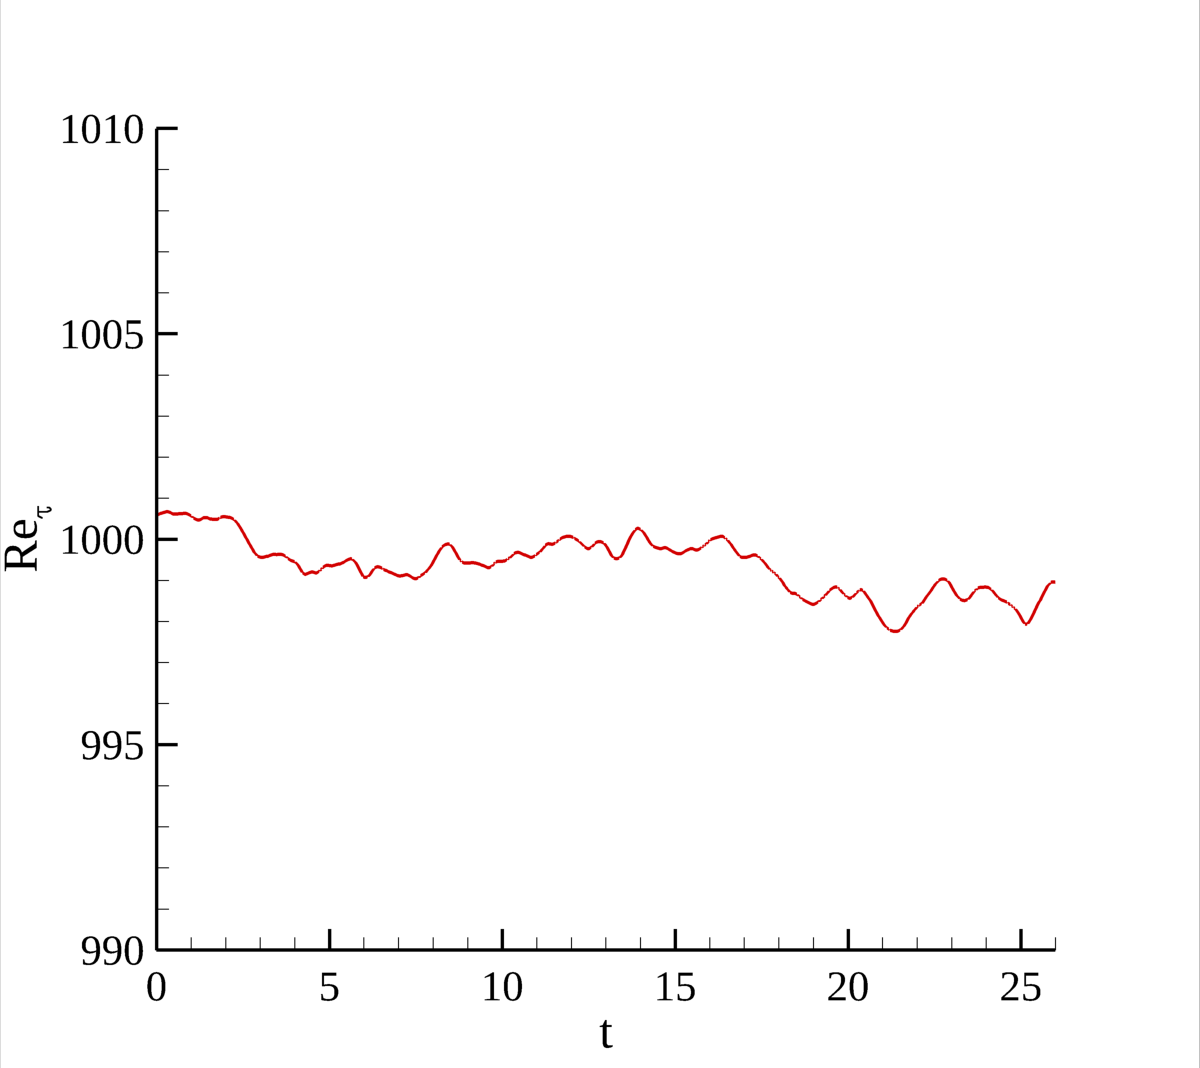
\includegraphics[width=5.00in]{./figures/re_tau.png}
 \caption{Friction velocity Reynolds number during the channel flow simulation during the database time interval}
 \label{fig:re_tau}
\end{figure}

\begin{figure}[h]
  \centering
  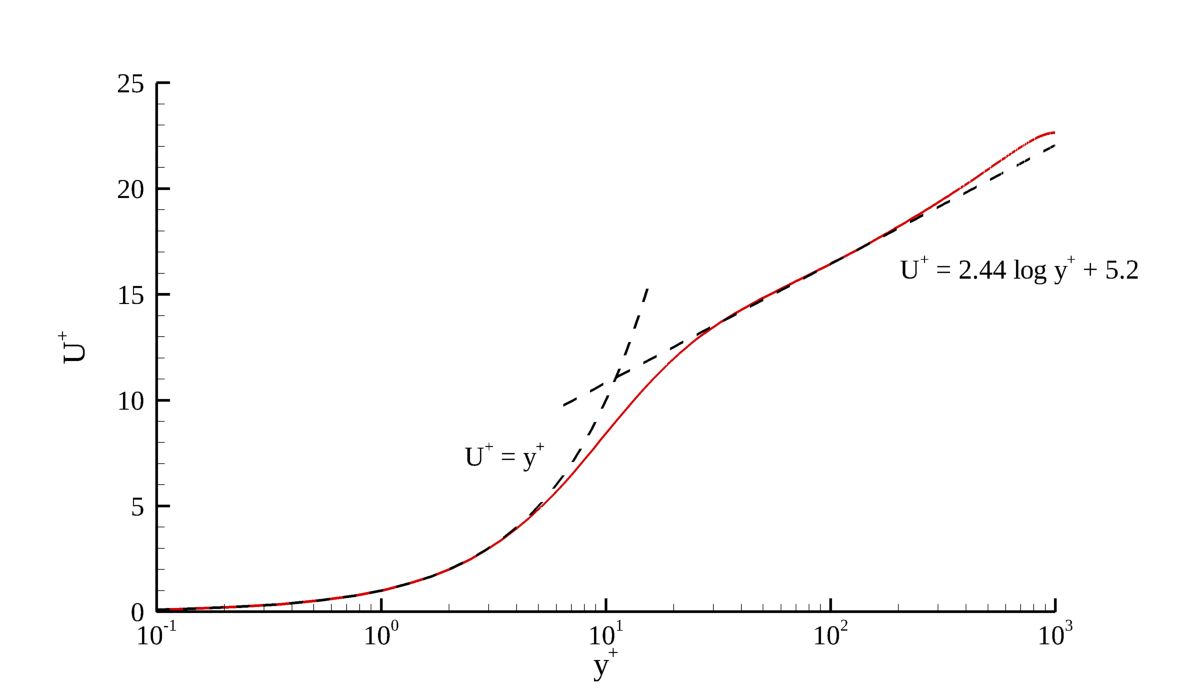
\includegraphics[width=7.00in]{./figures/u.png}
  \caption{Mean velocity profile in viscous units. Standard values of $\kappa=0.41$ and $B=5.2$ are used in the log-law (dashed line) for reference.}
 \label{fig:u}
\end{figure}

\begin{figure}[ht]
\centering
\begin{minipage}[b]{0.45\linewidth}
  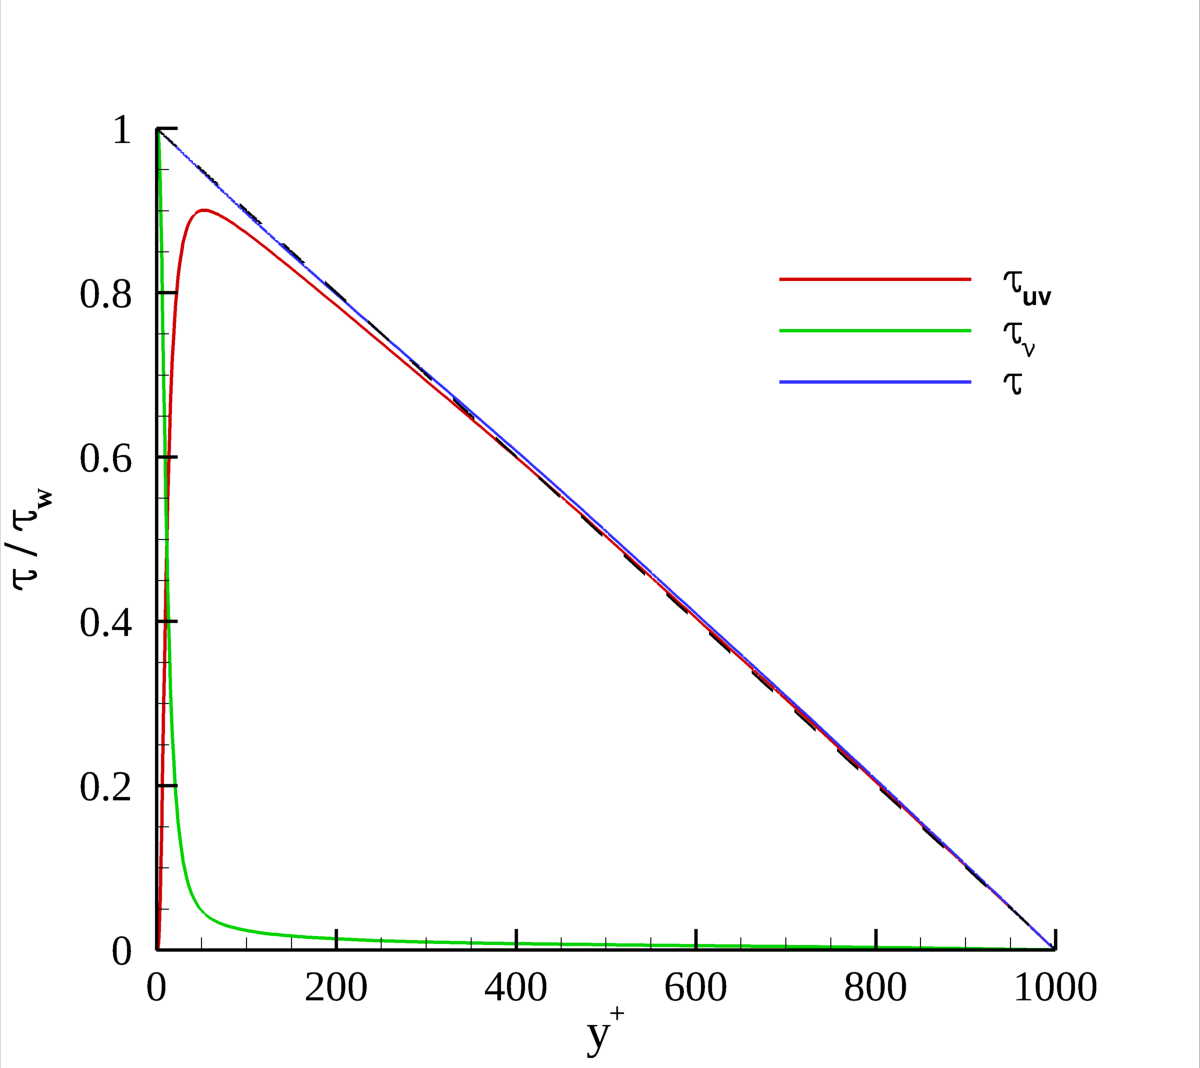
\includegraphics[width=3.37in]{./figures/tau.png}
  \caption{Mean viscous, turbulent, and total shear stress normalized by the wall stress}
  \label{fig:tau}
\end{minipage}
\quad
\begin{minipage}[b]{0.45\linewidth}
  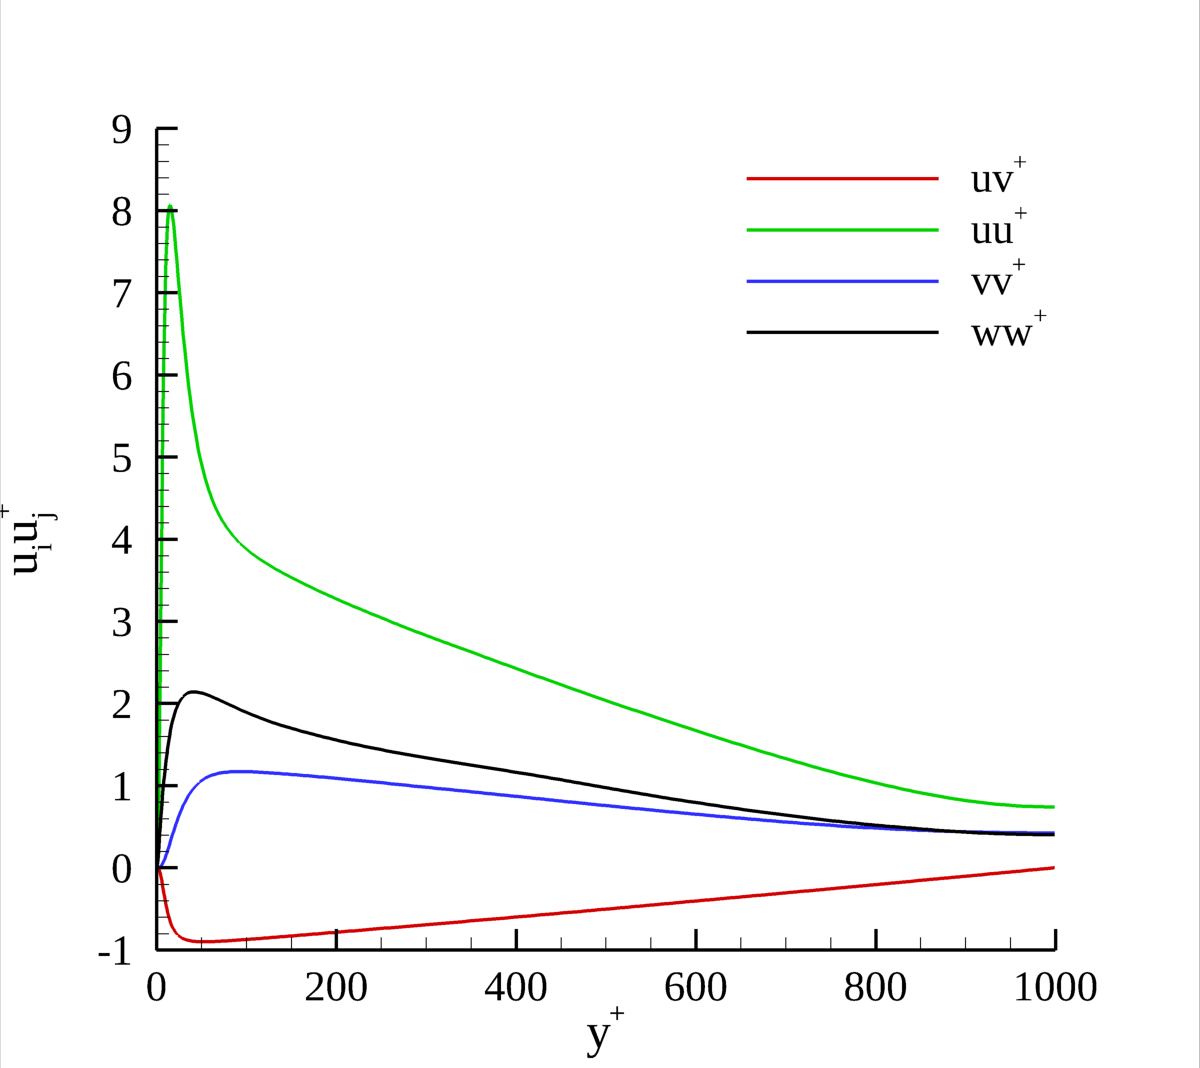
\includegraphics[width=3.37in]{./figures/rs.png}
  \caption{Velocity covariances in viscous units}
  \label{fig:rs}
\end{minipage}
\quad
\begin{minipage}[b]{0.45\linewidth}
  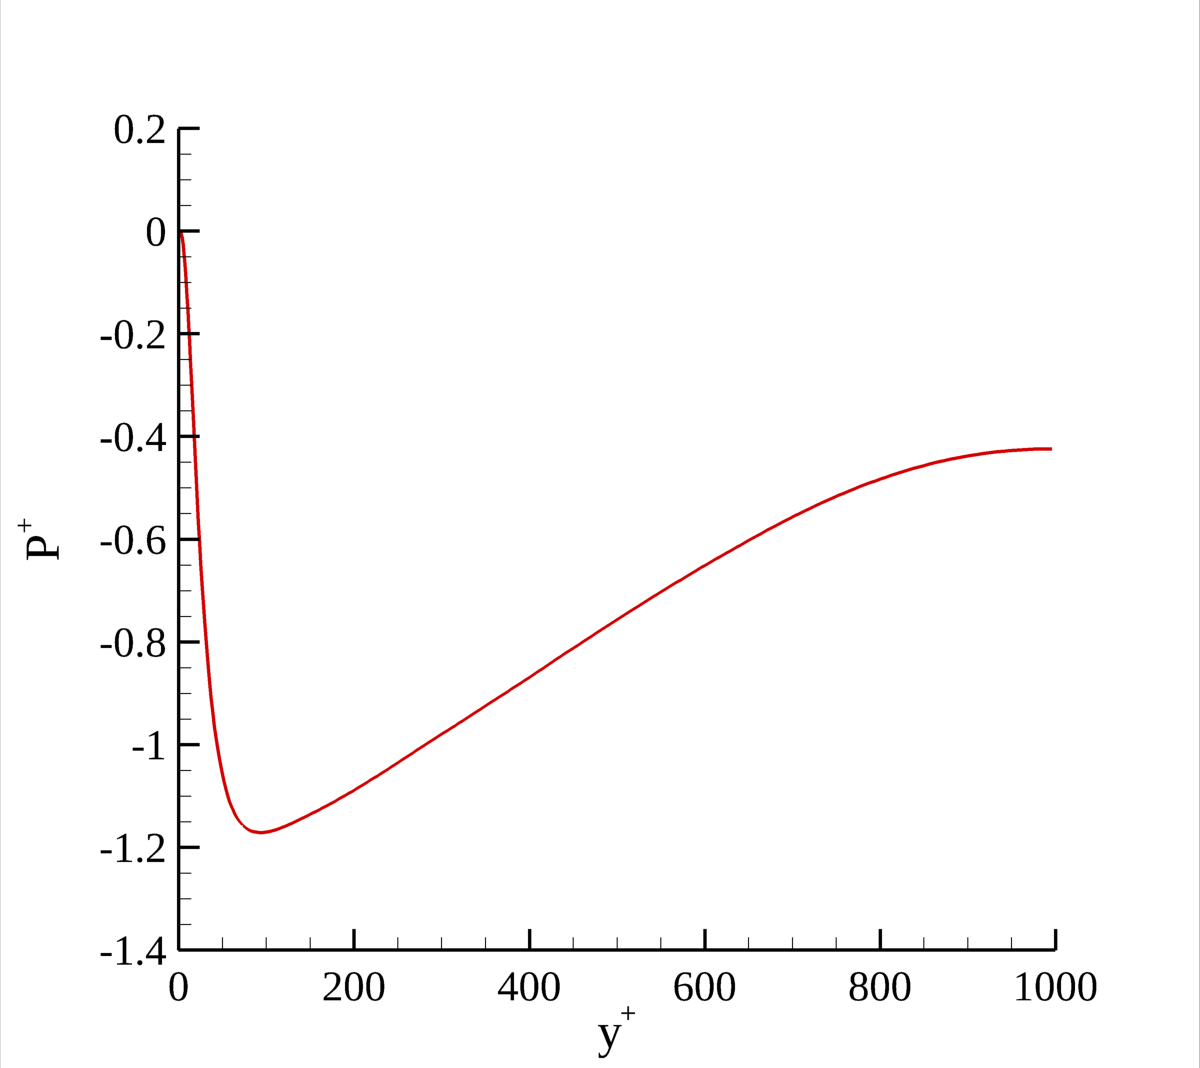
\includegraphics[width=3.37in]{./figures/p.png}
  \caption{Mean pressure profile in viscous units}
  \label{fig:p}
\end{minipage}
\quad
\begin{minipage}[b]{0.45\linewidth}
  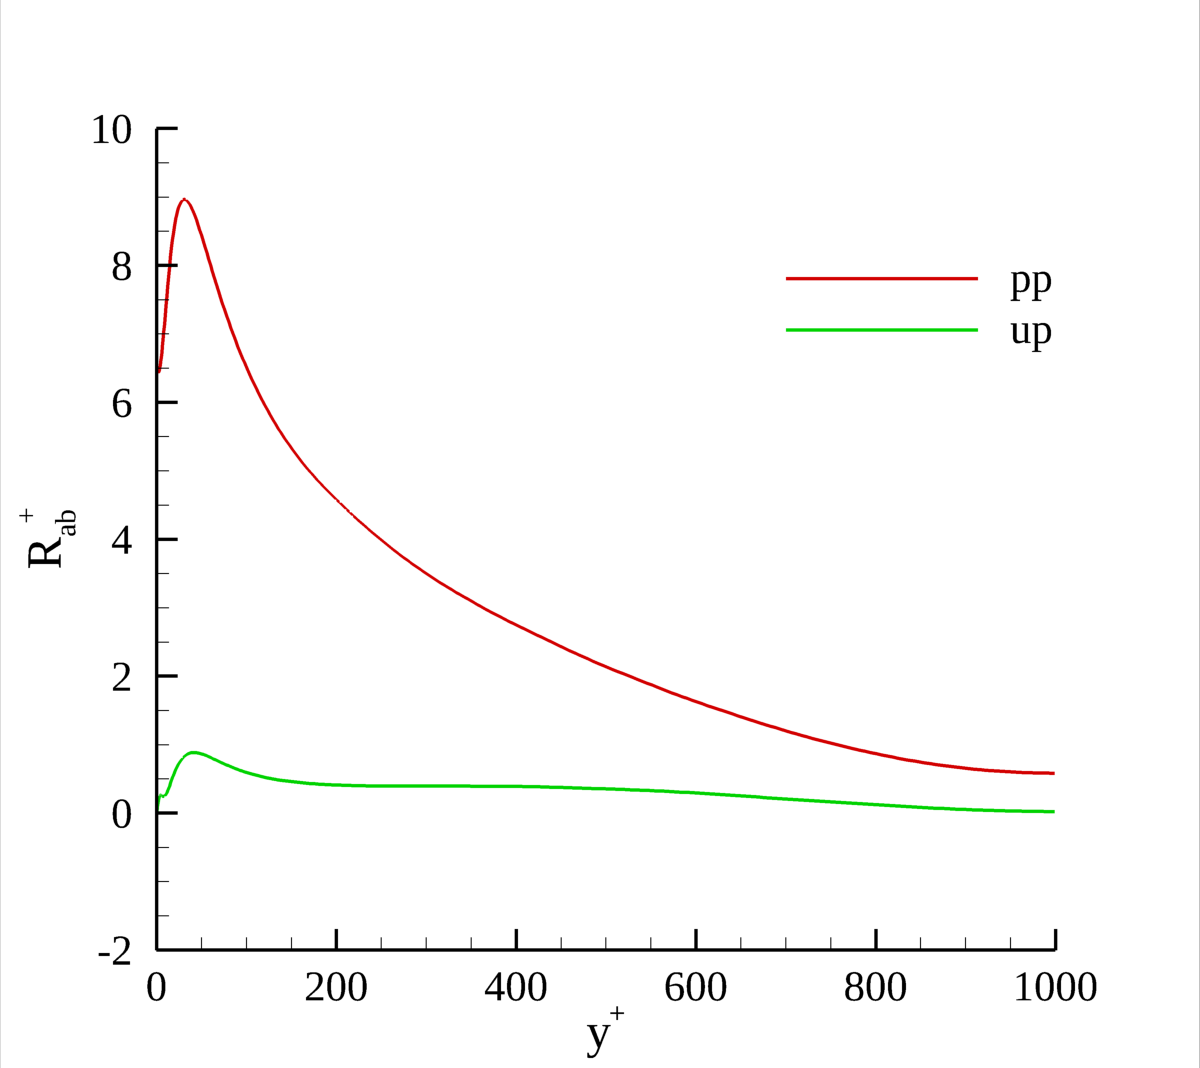
\includegraphics[width=3.37in]{./figures/velp-covar.png}
  \caption{Pressure variance and pressure-velocity covariance in viscous units}
  \label{fig:velp-covar}
\end{minipage}

\end{figure}

\begin{figure}[ht]
  \centering
  \subfigure[$y^+ = 10.11$]{%
    \includegraphics[width=2.78in]{./figures/{spectra-kx-yplus-10.11}.png}
    \label{fig:spectra-kx-1}}
%  \quad
  \subfigure[$y^+ = 29.89$]{%
    \includegraphics[width=2.78in]{./figures/{spectra-kx-yplus-29.89}.png}
    \label{fig:spectra-kx-2}}
  \subfigure[$y^+ = 99.75$]{%
    \includegraphics[width=2.78in]{./figures/{spectra-kx-yplus-99.75}.png}
    \label{fig:spectra-kx-3}}
%  \quad
  \subfigure[$y^+ = 371.6$]{%
    \includegraphics[width=2.78in]{./figures/{spectra-kx-yplus-371.6}.png}
    \label{fig:spectra-kx-4}}
%  \quad
  \subfigure[$y^+ = 999.7$]{%
    \includegraphics[width=2.78in]{./figures/{spectra-kx-yplus-999.7}.png}
    \label{fig:spectra-kx-5}} %
  \caption{Streamwise power spectral densities at various $y^+$ locations as function of $k_x$}
  \label{fig:spectra-kx}
\end{figure}

\begin{figure}[ht]
  \centering
  \subfigure[$y^+ = 10.11$]{%
    \includegraphics[width=2.78in]{./figures/{spectra-kz-yplus-10.11}.png}
    \label{fig:spectra-kz-1}}
%  \quad
  \subfigure[$y^+ = 29.89$]{%
    \includegraphics[width=2.78in]{./figures/{spectra-kz-yplus-29.89}.png}
    \label{fig:spectra-kz-2}}
  \subfigure[$y^+ = 99.75$]{%
    \includegraphics[width=2.78in]{./figures/{spectra-kz-yplus-99.75}.png}
    \label{fig:spectra-kz-3}}
%  \quad
  \subfigure[$y^+ = 371.6$]{%
    \includegraphics[width=2.78in]{./figures/{spectra-kz-yplus-371.6}.png}
    \label{fig:spectra-kz-4}}
%  \quad
  \subfigure[$y^+ = 999.7$]{%
    \includegraphics[width=2.78in]{./figures/{spectra-kz-yplus-999.7}.png}
    \label{fig:spectra-kz-5}} %
  \caption{Spanwise power spectral densities at various $y^+$ locations as function of $k_z$}
  \label{fig:spectra-kz}
\end{figure}


\end{document}
